\documentclass{article}
\usepackage[utf8]{inputenc}
\usepackage{xspace}
\usepackage{fancyhdr}
\pagestyle{fancy}
\fancyhf{}
\usepackage{listings}
\usepackage[]{graphicx}
\usepackage[toc,page]{appendix}
\usepackage{geometry}
\usepackage{hyperref}
 \geometry{
 a4paper,
 left=30mm,
 top=22mm
 }
\rfoot{\thepage}
\lfoot{Paris Physics Master - Stage Report}
\renewcommand{\headrulewidth}{0pt}

\title{\textbf{LHAASO Detector Simulation\\ \large{Machine Learning Classification of High Altitude Particle Showers }}}

\author{Stage Report: APC Laboratoire\\ 2020-2021}
\date{Presented by David Paipa \thanks{Sorbonne Université. Paris Physics Master 2020-2021 . Paris, France}\\
\small{Supervised by Andrii Neronov\thanks{Laboratoire APC - Université Paris Diderot. Paris, France}}
}

\begin{document}
\maketitle
\vspace{10cm}
\begin{center}
\textbf{ June 21, 2021 }   
\end{center}
% \newpage

% \textbf{Version control}
% \vspace{1cm}


% \begin{tabular}[h!]{|p{1.5cm}|p{1.5cm}|p{5cm}|p{4cm}|}
% \hline
%   \textbf{Version number}   & \textbf{Date issued} & \textbf{Authors} & \textbf{Update information} \\
%   \hline
%   \textbf{V1.0}  & month 2021 & Name surname (number) 
   
%   name surname (number) 
   
%   name surname (number) 
   
%   name surname (number) 
   
%   supervision: prof. name & Original version of the script \\
%   \hline
%   & & & \\
%   \hline
%   & & & \\
%   \hline
%   & & & \\
%   \hline
%   & & & \\
%   \hline
% \end{tabular}

\newpage

\tableofcontents
\newpage



\section{Introduction}
\subsection{Context}

\subsubsection{Cosmic Rays and Gamma Rays}
The universe is a diverse and chaotic environment, yet cold and relatively quiet. In the core of violent events, such as supernovas or a black hole eating an unfortunate star, Highly energetic photons are emitted from charged particles that are being accelerated to extremely high energies. Its important to know that other particles such as protons, electrons, positrons, and atomic nuclei are also adrift in the vastness of space at high velocities, along with the photons coming from stars, Interstellar medium and highly energetic sources. \textbf{Cosmic Rays} are protons and nuclei moving at high velocities and originated outside the earth, \textbf{Gamma Rays} on the other hand, are highly energetic photons (from $\sim 10^{6} - > 10^{15} $) emitted as well from extraterrestrial and even extragalactic sources.
 About 90\% of cosmic rays are protons, 9\% are alpha particles, and the remaining ~1\% are other particles.

When traveling through interstellar space, the low density makes collisions extremely unlikely, but when the cosmic and gamma rays arrive to earth's atmosphere, the cross-section increases due to the density of the medium, the air, eventually unleashing a particle shower event: an \textbf{Extensive Air Shower (EAS)}.  Constantly cosmic and gamma rays are colliding with the high atmosphere, creating EAS on earth's sky in a regular basis, the detailed study of the spectra and of these events should give information about the extreme events happening in the sources.
\subsubsection{High Altitude Extensive Air Showers}
Once a \textbf{primary particle}, cosmic or gamma ray, impacts the high atmosphere, the initial collision has in its center of mass a very high energy, which results in the creation of more particles, initiating a chain reaction that stops when hitting ground or when the energy of the created particles in a collision is not enough to create a pair of new particles.   

Observations and models, such as the Heitler model for EAS \cite{heitlerarticle},
show that particle showers originated by gamma photons (GS) are different than the originated by protons or hadrons (PS) in structure and particle densities at the ground level, after the shower particles have crossed several mean free path lengths. Figure \ref{fig:difergp} illustrates this difference in the structure of GS and PS.

 \begin{figure}[!h]
    \centering
    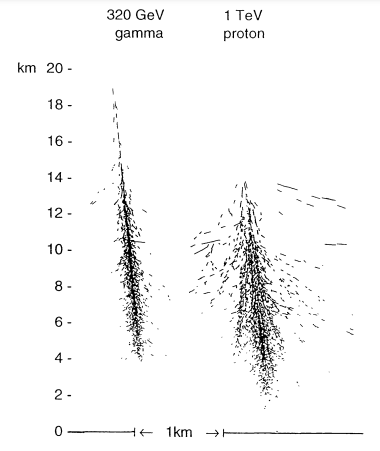
\includegraphics[width=0.5\textwidth]{imgs/showersdif.PNG}
    \caption{Different form of gamma and proton induced showers. The left shows a 320GeV gamma induced EAS and the Right shows a 1TeV proton induced EAS.The lateral scales is exagerated by a factor of 5. Image and caption taken from the original publication \cite{differencesgp}}
    \label{fig:difergp}
\end{figure}
The events differ since the initial particle production, where GS generate an electron-positron pair and PS generate charged and neutral pions. In the GS, the subsequent collisions lead to more photons and charged particles in a nearly symmetric distribution, while in the PS the charged pions initiate what can be seen as secondary particle showers and the neutral pions decay before interacting, leading to minor electromagnetic subshowers. The result is a more spatially extensive particle shower for PS, as observed in figure \ref{fig:difergp}, under the mechanisms exposed in Figure \ref{fig:difergp_heitler}

 \begin{figure}[!h]
    \centering
    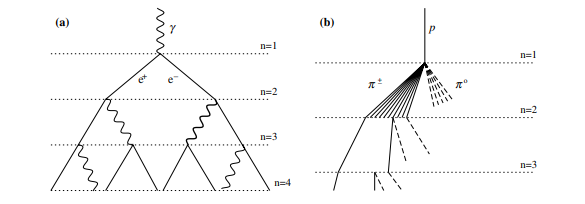
\includegraphics[width=0.9\textwidth]{imgs/showersdif_heit.PNG}
    \caption{Schematic views of (a) an electromagnetic cascade and (b) a hadronic shower. In the hadron shower, dashed lines indicate
neutral pions which do not re-interact, but quickly decay, yielding electromagnetic subshowers (not shown). Not all pion lines are
shown after the n = 2 level. Neither diagram is to scale. Image and caption taken from the original publication \cite{heitlerarticle}}
    \label{fig:difergp_heitler}
\end{figure}

\subsubsection{High Energy Astronomy}
When talking about astronomy, we are interested in the photons coming form extraterrestrial sources. In this case at high energies,  these are the gamma rays that can be detected from earth. The energy of such photons is above 0.1MeV and, as we will discuss in the next sections, they have been detected in energies up to 1.4PeV \cite{UHEgammapaper}. In the case we will discuss we are interested in photons with energries in the order of 100TeV.

Up to today collaborations and experiments like LHAASO and TIBET are arriving to amazing conclusions thanks to the Ultra high energy astronomy, such as the First Detection of sub-PeV Diffuse Gamma Rays from the Galactic Disk \cite{TIBETpaper} or the previously mentioned cased of the photon with the highest energy measured at 1.4PeV, leading to the formulation of a new kind of source. To do astronomy with accurate data of radiation emitting sources, it is fundamental to differentiate between gamma and hadron induced showers, since we are interested in the first. Researchers report obtaining proton discrimination errors under 1/$10^4$, having on average a PS misclassified every 10,000. 

\subsubsection{LHAASO}
The \textbf{Large} \textbf{H}igh \textbf{A}ltitude \textbf{A}ir \textbf{S}hower \textbf{O}bservatory
AS specified by the LHAASO collaboration\cite{LHAASOpaper}  is a new generation
instrument targeting a deep investigation of the High Energy Universe.LHAASO is located at high altitude (4410 m a.s.l. [29  21  31 N, 100 08 15 E]
in the Daochen site, Sichuan province, P.R. China.
The first phase of LHAASO consist of the following major components, and they can be visualized in Figure \ref{fig:lhaasodesign}:
\begin{itemize}
    \item 1$km^2$ array (LHAASO-KM2A) for electromagnetic particle detectors (ED, refered as EM in this report), 1$m^2$ each in size,
divided into two parts: a central part including 4901 scintillator detectors (15m spacing) to cover
a circular area with a radius of 575 m and an outer guard-ring instrumented with 294 EDs (30 m
spacing) up to a radius of 635 m.
 \item An overlapping 1$km^2$ array of 1171 underground water Cherenkov tanks 36$m^2$ each in size, with
30 m spacing, for muon detection (MD, total sensitive area 42,156 $m^2$).
 \item A close-packed, surface water Cherenkov detector facility with a total area of about 78,000 $m^2$
(LHAASO-WCDA).
 \item 20 wide field-of-view air Cherenkov telescopes (LHAASO-WFCTA).
\end{itemize}
as far as this stage report is concerned, the grids we are focusing are the EM scintillator grid and the MD muon detector grid. The temporal resolution of LHAASO is around a couple nanoseconds. Amongst some of the results LHAASO expect to get within the collaboration observations are:
\begin{itemize}
    \item Studying the acceleration mechanism of sources of Ultra high energy photons
    \item perform an unbiased sky survey of the northern sky with energy ranges from sub-Tev to 100Tev
    \item LHAASO will allow the reconstruction of the energy spectra of different cosmic ray mass groups
in the range $10^{13} – 10^{18}$ eV with \textbf{unprecedented statistics and resolution}.
\item LHAASO will allow important studies of fundamental physics
(such as indirect dark matter search, Lorentz invariance violation, quantum gravity) and solar and heliospheric
physics. Checking for anomalies in the TeV spectra of Blazars looking for Lorentz invariance violation could lead to interesting conclusions on Quantum Gravity Models.


\end{itemize}



\subsection{Motivation for this research}
LHAASO is opening available a new window of high energy observations of the universe in the range 100-1000TeV, with potential to collect data that point to new physical phenomena. For example, The observation of the tail of the spectra of $\gamma$-ray sources is expected to unveil new information about the acceleration mechanism of the $\gamma$-ray emitting particles at energies over 1PeV. LHAASO will also provide data to map the Galactic diffuse gamma-ray emission above few hundreds GeV, enabling new studies in cosmic ray physics and gamma-ray astronomy.  

To do such amazing new projects, a necessary basis is a solid database of the EAS, specifically being able to tell which is the particle that initiated the shower so astronomical observations are accurate. Furthermore, researchers need to make this classification automatically given the huge amount of data available from the observatories. 

Finding a way of selecting Gamma events in this observations is the first step when gathering new data that supports (or not) claims of Physics beyond the standard model and not identified gamma sources in space. Good and more sophisticated classification algorithms are already in use but setting up these \textit{Toy models} Help to understand better potential flaws or advantages. Playing a little with the detector's properties might also give new information on methods to classify High energy events.
\subsection{Objectives}
The objectives planned for the internship are:
\begin{itemize}
    \item Understand and domain the use of CORSIKA to simulate EAS under tuned conditions. Build example databases for model training.
    \item Simulate two grids of detector arrays resembling the LHAASO muon detector array and electromagnetic scintillator array. Use the generated EAS to simulate readings  made by LHAASO on the ground.
    \item Understand the underlying difference between EAS induced by PS and by GS. Use this information to select a learning model that can classify the primary particle of the EAS according the the detectors' information. 
    \item Extract information from simulating numerous initial energies of the primary particle and determine how this information may be induced using the detector data available.
    \item Create a model that favors the correct classification of PS, since is the data we want to filter from the GS data used in astronomy. Try to replicate the results obtained in \cite{UHEgammapaper} where they report an error fraction of $10^{-4}$ when classifying PS.  
    
\end{itemize}


\section{Tools and Data}
\subsection{CORSIKA software}
\textbf{CO}smic \textbf{R}ay \textbf{SI}mulations for \textbf{KA}scade\cite{CORSIKA} is a software written in FORTRAN 77 for simulating extensive air showers induced by high energy collisions of cosmic rays in the high atmosphere. It can simulate a wide range of initial energies, from the order of $\sim$1 TeV ($10^{12}eV$) up to $\sim$100 EeV ($10^{20}eV$).

CORSIKA works by creating MonteCarlo simulations of Extensive Air showers taking into account atmospheric Neutrinos, Hadron interactions, Electromagnetic interactions, Cherenkov radiation, Strong interactions at low energies, Nuclear fragmentation, accurate cross-sections among other physical phenomena. Most of these interactions come in packages that can be installed in the creation of the executable.  

The process for running a simulation is the following:
\begin{itemize}
    \item Execute the  setup installer \footnote{Named "coconut" by the authors} to create an executable file. In this step the CORSIKA tools and packages are defined.
    \item Create a text file in the correct format to input the simulation parameters. We will discuss this simulation parameters below.
    \item Run the executable file with the text file as the input. This will start CORSIKA and create DATXXXX output files in the folder set by the user.
\end{itemize}

This last DATXXXX file is the one we care about. This binary file contains the information \textbf{per shower} of each particle that hit the ground\footnote{Particle properties are xy-coordinates , the 3 momentum components , the type of particle and the time when hitting the ground at the defined observation altitude.}. 

CORSIKA can be installed with a lot of complementary models of hadronic and EM interactions at different energy regimes. some of these packages like GHEISHA\footnote{Hadronic interactions at lower energies are described either by the more
sophisticated GHEISHA interaction routines or the rather simple ISOBAR model}, EGS4, QGSJET, DPMJET\cite{dpmjet}\footnote{DPMJET and QGSJET for example allow the simulation of hadron-hadron, hadron-nucleus, nucleus-nucleus, photon-hadron, photon-photon and photon-nucleus interactions in a wide range of energies} can enhance the calculation of physical effects in the EAS by implementing updated values, cross-sections and interaction models.In this case we are using CORSIKA 77400 with GHEISHA, DPMJET, QGSJET,EGS4,Cherenkov radiation as some of the featured complements of CORSIKA. More specific models add relatively small corrections to the particle data.



\subsection{Dante cluster at APC}
While working on the internship I was provided with access to the HPC infrastructure at APC Laboratoire. DANTE is a cluster working with Slurm, where each node\footnote{There are two types of nodes but during the internship I used only the regular sized. more information can be found at \url{si-apc.pages.in2p3.fr/dante-cluster/}} counts with 40 CPU and 96 Gigabytes of RAM. This Tool will enhance the calculation velocity and reduce drastically the computing time. Information on its performance and use is described in further sections.
\subsection{Machine learning and statistical concepts}


\subsubsection{statistics}
\paragraph{features and target.} A learning model works by taking a set of examples, each example made of features (characteristics of the observation) and a target (the class of the observation), and learning from the statistical patterns among features to predict the correct classes.When the model learned, or trained, it can now receive any set of features and predict the associate target. With more examples provided on the training, the model is more \textbf{accurate} on the classification. The target in this case is a binary target, since there are only two possible classes.
\paragraph{Correlation and covariance.}
Covariance measures the degree of linear relation among two  random variables or, in this case, sets of data in one dimension. It shows whether the behavior of one variable can be linearly dependent, to some degree, on the other variable. The range of the covariance is not normalized, which is a problem because it depends on the magnitudes of the variables.  

The pearson correlation can be seen as a normalized covariance. Is defined as the covariance divided by the product of the deviations of the two sets. The range of the correlation coefficient is between -1 (strong negative relation) and +1(strong positive relation), being 0 associated to non-correlated data.Is a way of checking the dependence (in magnitude and direction) between these two sets and is useful to point at causal relationships among data or detect predictive relationships that can be exploited. 

This calculations can be seen in some cases as  \textit{a priori} measurements of how a prediction model would perform  on a data set ,given how well the features explain the behavior and variance of the target.



\paragraph{Metrics.} When predicting a binary target, of positive and negative cases, with a classification model, some metrics arise from comparing the expected results with the results obtained by the model. The confusion matrix shows the total incidences in each of the four cases : positive cases correctly classified (true positives), positive cases misclassified as negatives (false negatives) , negative cases correctly classified (true negatives) and negative cases misclassified as positives (false positives) .These are often refered as tp,fn,tn,fp.

The \textbf{accuracy} is the proportion of correctly classified cases over the total cases. The \textbf{recall} is the proportion of positives that were correctly classified over the total number of positive cases, while \textbf{sensitivity} is the proportion of negative cases that were correctly classified. The \textbf{precision} is the the proportion of the positive cases correctly classified over the total cases predicted as positive. Wrapping up:
\begin{equation}
    acc =  \frac{tp+tn}{tp+tn+fp+fn}
\end{equation}
\begin{equation}
    recall =  \frac{tp}{tp+fn} 
\end{equation}
\begin{equation}
    sensitivity =  \frac{tn}{tn+fp} 
\end{equation}
The F1 score is the harmonic mean of precision and recall, and is a metric of the predictor's accuracy ranging form 0 to 1, defined as:
\begin{equation}
    F1 = 2\cdot \frac{precision \cdot recall}{precision + recall}
\end{equation}


\paragraph{Logistic Regression}
A linear regression allows to find a linear combination of features to obtain a value relatively close to the target in the case of a continuous target. In the case of binary targets,0 or 1, it is better to use a logistic regression, which can map a set of features to a single real number between 0 and 1. The model comes from the logistic function in n-dimensions:
\begin{equation}
    R_c = c_0  + c_1\cdot x_1 + c_2\cdot x_2 + c_3\cdot x_3+...+c_n\cdot x_n
\end{equation}
\begin{equation}
 P(X) = \frac{1}{1 + e^{-R_c}}
\end{equation}
where each $x_i$ is the i-th variable and $c_i$ is a  constant coefficient. Not how $R_c$ can be any real value, but the envelope of the logistic function restricts its value to a probability $P(X)$ between 0 and 1. This is the probability of being a target in the class of 1.  The logistic model in order to convert the probability into a class takes the $P(X)$ and compares it with a threshold value: if  $P(X)$ is above the threshold the observation is classified as a positive case, as 1. If not, it is classified as a negative case, as 0.


Some other predictive models are:
\begin{itemize}
    \item \textbf{Decision Tree} A model that splits the feature space into regions using binary decisions, assigning a class to each region.
    \item \textbf{Random Forest} An ensemble of decision trees implemented as predictive voters of a bigger model.
    \item \textbf{Support Vector Classifier} A model that defines boundaries in the feature space by maximizing the distance between the boundaries and the data points.
    \item \textbf{Polynomial regression} linear regression assuming a target dependence on the features with different exponential degrees above 1.
\end{itemize}

\section{Development}
The process to follow, according to the objectives, is subdivided into two major tasks: The first is \textbf{mimicking} the LHAASO detector readings by simulating the particle showers and the in-ground detectors, this can be achieved with the help of CORSIKA and HPC. The second task is taking the generated data and find patterns that can be used to classify the shower events according to its primary particle. This might be tricky because, as we will see, we might want to penalize one type of misclassification more than the other. In this section I will present the main results obtained during the stage, the intuition behind them, and the obstacles presented during the development of each phase.

\subsection{CORSIKA: generating High altitude particle showers}
To obtain accurate predictions of the readings that LHAASO may receive its important to have a big sample of simulated events. With more events, the learning algorithm will have more examples to learn the patterns in the data. Furthermore, more data implies more objective metrics for the algorithm's performance.

We are interested in the classification of EAS caused by protons or by gamma photons, so these will be the cases simulated. Since we want to have an objective view of the data behavior, the number of simulated cases is balanced (same number of proton and gamma showers).

\subsubsection{Setting the simulation parameters}

\paragraph{Simulation.}
The output directory, number of showers simulated and file name are changed according to the case. The seeds are always changed among simulations to promote random behavior and variety of cases. 
\paragraph{Initial reaction}
The primary particle is set according to the batch simulated. The initial energy boundaries is set as an energy range, with a energy slope, this being the exponential critical coefficient of the energy density distribution. since its exponential a slope of 1 would give a uniform distribution while a slope of 2.7 would results in more events of lower energy (within bounds) than event of high energy.
\paragraph{Environment.} To simulate the event reading at LHAASO the height of evaluation is set to be at $44\times 10^4$ cm. The angles of incidence are restricted to incident particles coming from the zenith. Take into account that in a real case the particles are coming from any direction in the sky.
\subsubsection{Simulated cases}
The whole constructed event database has 1600 shower events (800 of each class) and the respective simulated batches are labeled as following:

\begin{table}[h!]
\centering
\begin{tabular}[]{c cccc}
\hline

  \textbf{Label}   & \textbf{\# Showers} & \textbf{E. range inf.} & \textbf{E. range sup.} & \textbf{E. slope}  \\
  \hline
  \hline
  350batch & 350 each & 5 & 500 & -2.7 \\
  150show50Tev& 150 each & 40 & 60 & -1 \\
  150show100Tev& 150 each & 90 & 110 & -1 \\
  150show150Tev& 150 each & 140 & 160 & -1 \\
  \hline
\end{tabular}
    \caption{Data batches simulated in CORSIKA. The 1600 examples used for the prediction model is the concatenation of all events simulated and listed here. In the shower number definition \textit{each} means a balanced sample of proton and photons showers. The energy ranges are given in TeV.}
    \label{tab:datalabels}
\end{table}

The performance of the cluster was evaluated generating 1,10,100 and 1000 proton showers under the conditions presented in appendix \ref{filecorsika}. The results of processing time and output file size are shown in figure \ref{fig:DANTEperformance}


At the end of the execution, a file in the format \textit{DATXXXXX} is generated containing the information of the simulation and, for each shower, the information of the particles that arrived to the ground. This file has a considerable Memory size for a few hundreds of showers as seen in figure \ref{fig:DANTEperformance}, and may increase drastically if the initial energy increases. The binary output files from CORSIKA are extracted into an array of particle objects, having  information on its properties and which shower each particle belongs to. 

\subsection{Simulating LHAASO detectors}
Now the goal is to simulate an accurate ground detector with the specifications of LHAASO. we are interested in simulating two detector grids: the LHAASO-KM2A for electromagnetic particle detectors (ED) and the array of muon detectors (MD)  composed of  water Cherenkov tanks.

I used a object-oriented structure in python to create a script that allows the creation of a detector grid in which the grid geometry and detector properties can be defined by the user. With this, I created each of the two overlaped triangular grids with the specifications given before, resulting in the detector array displayed on figure \ref{fig:detectorarray}

 \begin{figure}[!h]
    \centering
    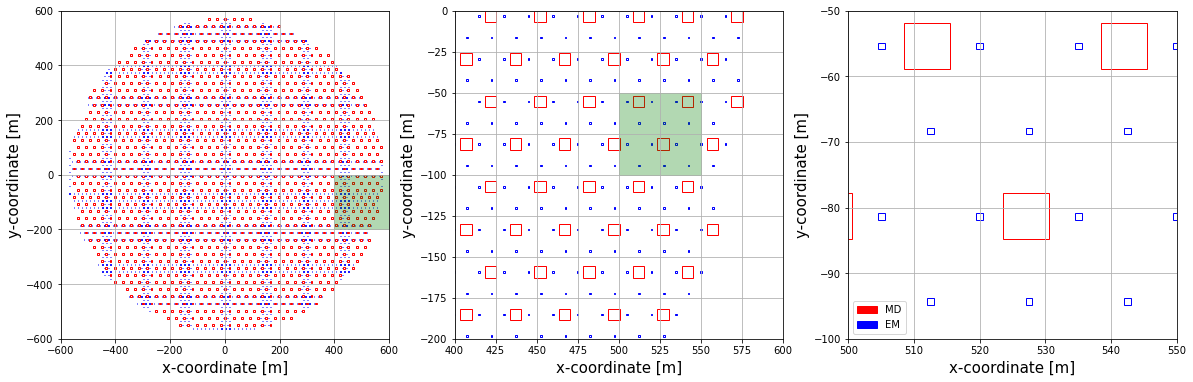
\includegraphics[width=\textwidth]{imgs/detect_array_lhaaso.png}
    \caption{These are the simulated detector objects represented in the ground plane. The number of EM and MD in LHAASO are 4901 and 1171 respectively, and for the simulated array are 5324 and 1330.}
    \label{fig:detectorarray}
\end{figure}

The minimal object in this object-oriented structure is the \textbf{detector} object. It is defined as a square box with some position for its center and a side length. The user can also define the \textbf{types of particles} that interact with the detector as well as an \textbf{energy threshold} for detection. 

The construction of the grid is relatively simple from here: once defined the \textit{detector} objects, \textit{line of detectors} objects are defined as a group of detectors and the whole \textit{grid} objects is a group of \textit{line of detector} objects. 

Each \textbf{line of detectors} has an initial point, a length, a phase and a separation length. The line goes form the initial point towards positive y-coordinate for its corresponding length. The first detector is placed on the phase value and the others are placed with a constant separation length of the value previously defined. This separation is set according to the separation between lines to form the triangular grid.

When the grid is constructed it needs a set of particle names to which all detectors are sensible as well as the energy threshold for detection. The grid is also provided with a name to have \textit{traceability} of the particle detection. In the case of the LHAASO grid simulated, the names of the grids are \emph{em\_scintillator\_array} and \emph{muon\_detector\_array}.
The characteristics of these grids are displayed in table \ref{tab:gridchars}

\begin{table}[h!]
\centering
\begin{tabular}[]{c|ccccc|ccccc}
\hline
  & \multicolumn{5}{c}{LHAASO}  & \multicolumn{5}{c}{Simulated} \tabularnewline
\hline
   Grid Name & \textbf{$R_G$} &\textbf{$S_G$} & \textbf{$L_D$} & \textbf{$D_G$} & \textbf{$E_{th}$} & \textbf{$R_G$} & \textbf{$L_D$} &\textbf{$L_G$} & \textbf{$D_G$} & \textbf{$E_{th}$} \\
  \hline
  em\_scintillator\_array & 575m & 15m & 1m & 4901 & - & 575m & 15m & 1m & 5324 & 3 Mev \\
  muon\_detector\_array & 575m & 30m & 7m & 1171 & 1.3Gev & 575m & 30m & 7m & 1330 & 1.3Gev \\

  \hline
\end{tabular}
    \caption{Attributes of the LHAASO EM and MD grids compared to the simulated grids.$R_G$ is the grid's area radius (circular geometry), $S_G$ is separation between detectors of the same grid, $L_D$ is the length of size of each detector (square), $D_G$ is the number of detectors in the grid and $E_{th}$ is the energy threshold for each grid.}
    \label{tab:gridchars}
\end{table}


Each time a grid interacts with a particle set, this interaction is delegated from the object groups to each of the components, returning \textbf{True} when the particle is within the detection conditions. Each particle is assigned to the line with the closest x-coordinate and the detector with the closest y-coordinate in order to be verified. The particle is verified as detected by the closest detector if these \textbf{detection conditions} are valid:
\begin{itemize}
    \item The particle's xy-coordinates are within the range of the detector
    \item The particle is of the type to which the detector is sensible
    \item The particle's energy is \textbf{above} the energy threshold of the detector
\end{itemize}
When detected, a count is added to the counter of the corresponding detector grid. For each detected particle the xy-coordinates of the detector and the time of the particle detection are stored for further analysis. Take into account these are the values that are expected to  be measurable since the real detectors can count events and register time\footnote{Time can be measured in real detectors with a precision of the order of nanoseconds. The particle objects from CORSIKA register the time of the particle hitting the ground since the initial atmospheric collision.} but can't tell the energy of the incident particle, its momentum, its exact position  or its exact behavior. 

The particle objects are processed by each one of the detector grids, returning a smaller set of particle objects being these the ones detected by each grid. For a  particle object detected the attributes are:
\begin{itemize}
    \item \textbf{shower :} The shower number identificator that corresponds to the particle.
    \item \textbf{x,y :} The xy-coordinates of the center of the detector that registered the particle event.
    \item \textbf{time :} The time in nanoseconds since the first collision
    \item \textbf{grid name :} Name of the detector grid that detected the particle. This is stored for analyzing the data in the future.
\end{itemize}

The computing time of this process is till being optimized. Trying to process 350 showers with the current algorithm for simulating LHAASO is taking around 8 hours in one node at DANTE, and its comprehensible since we are testing thousands of particles with thousands of detectors, for each shower event. More than 350 showers would probably induce a memory error. This is the reason we only have 1600 events available for now and not more (ideally of the order of $\sim 10^4$). Events with high initial energy are slower to process since has a lot more particles at detection level. The increase in particle number can be explained with a Heitler model, exposed in  \cite{heitlerarticle}.

\subsection{Study the detector data}
Up to this point the data available consists in a set of particles per shower labeled with the time and position of detection. Since the goal is to characterize the whole particle shower, the data available is pivoted to obtain a table. This table contains a row for each shower and the columns are: The number identificator of the shower, the primary particle (the target we want to predict), the counts generated in each grid of detectors,  a quantity to measure spatial dispersion and other for temporal dispersion.

\paragraph{Spatial dispersion.} For each shower the standard deviation of the x and y coordinates of the detected particles are stored as $\sigma$x and $\sigma$y respectively. The spatial dispersion $\Delta$xy is defined as the product $\sigma$x $ \sigma$y. The logarithm (base 10) of this dispersion value is stored in the attribute \emph{dxy}.
\paragraph{Temporal dispersion.} The dispersion $\sigma$t is the standard deviation in the detection times of the particles that constitute the shower, the quantity $\Delta$t is also the logarithm of this dispersion and is stored as \emph{dt}.
\paragraph{Detector counts.} Each grid of detectors stores the number of particles detected for each shower. At the end of the LHAASO detection simulation we are left with two positive integers\footnote{In an average case we're expecting hundreds or even thousands of particles, depending on the initial energy. Take into account that 0 is a possibility, some measures are taken to avoid divergences in future calculations}, one for EM counts and one for MD counts,  and the logarithm value ($log_{10}(n+1)$) is stored in a variable with the same names of the detector grids.
\paragraph{origin.} The numerical CORSIKA identifier of the primary particle. 1 and 14 for photons and protons respectively.

\subsubsection{Exploring the data available}
The table previously described will be called the \textbf{events master table} and will always have a balanced sample between proton and photon induced particle showers. The first events master table generated has 700 rows (350 for each case) and corresponds to the data set \emph{350batch}. The other 3 batches listed in Table \ref{tab:datalabels} were generated in further stages, but can be concatenated with the first data set to have a 1600 row master table and give an objective view of the distributions. A visual exploration of the data is displayed in figure \ref{fig:dataexploration}.

\begin{figure}[!h]
    \centering
    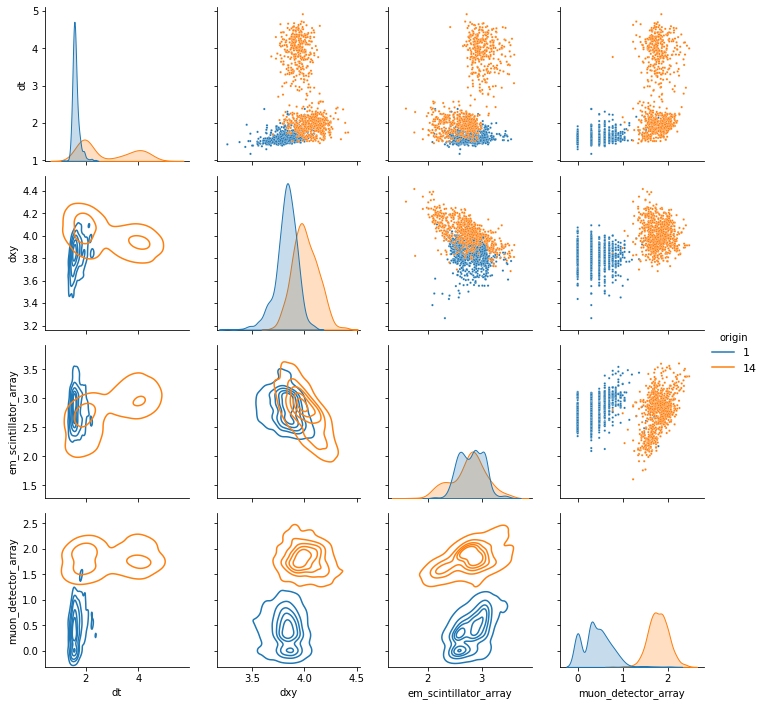
\includegraphics[width=0.9\textwidth]{imgs/data_exp.png}
    \caption{Visualization of the information in the event master table with 1600 showers (800 in each case).}
    \label{fig:dataexploration}
\end{figure}



Remind this is done in order to classify particle shower events according to the \emph{origin} attribute, so this must be the \textbf{target} of prediction for the model used. The other attributes of the shower $\Delta$t, $\Delta$xy, \emph{em\_scintillator\_array}, \emph{muon\_detector\_array} are used as \textbf{features} to predict the target.

The correlation and covariance of among features and between the features and the target is also calculated to observe the data behavior. The correlation and covariance matrices are displayed in figure \ref{fig:covcorr}.



In the data exploration a separation is visible in the feature space, corresponding to the two classes we want to predict. This means that any model used to classify this examples is most likely to draw a boundary separating the two diffuse\textit{clouds}, but since the groups are not totally exclusive a classification with a 100\% accuracy is impossible in a non-overfitted model. The KDE distributions in the diagonal of figure \ref{fig:dataexploration} shows that good parameters for separating the two clouds are \emph{muon\_detector\_array} and \emph{dt} since is among these axes that the distributions are less overlaped. In addition, we can see that in the planes  \emph{muon\_detector\_array} versus \emph{dxy} and \emph{muon\_detector\_array} versus \emph{em\_scintillator\_array}  the two cloud are more clearly separable than in the other cases. The correlation and covariance of the data shows a strong relation between the target and the features \emph{muon\_detector\_array} and \emph{dt}, implying that the distributions of these parameters explain the target distribution in the feature space.

\paragraph{Principal Component analysis.} In order to explore the feature space and the separation potential I tried using PCA to map the complete feature space of the master table. This analysis projects the data over the n-space (n is chosen) that contains most of the data variance. This is made through a linear transformation of the space based on the eigenvectors of the covariance matrix. By projecting the data over the n$=2$ space we can observe better the boundary between the two \textit{clouds} corresponding to each class. In figure \ref{fig:pca} this projection can be seen in detail with the data points distributed along the two principal components plane and a test of classification of this space performed by a Logistic Regression Model. In the projection the boundary between the two groups is more prominent but even this is affected by data points of one class being almost at the cloud center of the other class. The components in Table \ref{tab:pcacomp} can be seen as 2 vectors with 4 components each, that can be used to express any data point in the 4D space as a linear combination of this two vectors. The coefficients of each vector and their magnitudes are consistent with the results obtained in Figure \ref{fig:covcorr}  and Figure \ref{fig:covcorr_ener}, showing that \emph{dt} and \emph{muon\_detector\_array} have larger coefficients, implying high importance in the linear transformation.




The advantage of using PCA when the class clouds are relatively well separated is that the boundaries of classification can be fine tuned in a space where the separation is enhanced. PCA also can give information about the data variance, and in which quantity it can be explained by each one of the features. The disadvantage comes from the exercise of classification in practice. Since We want a model that can classify future events, each new set of features need to be transformed into the Principal components space by the same transformation, so this new future set can be classified under the same conditions as the examples. The same linear transformation matrix and the normalization coefficients\footnote{normalization understood as subtracting the mean from the data  and then dividing it by its standard deviation. The values of mean and deviation are calculated based on the examples given.} are necessary for this process and they depend highly on the examples given. PCA is a good way of exploring the data space, but since in this case  we are dealing with constantly increasing experimental data implementing PCA is not efficient.

\subsubsection{Dependence on energy of the primary particle}
An additional analysis on the characteristics of the showers is the study of how the master table changes for different ranges of initial energy regimes for the primary particle. for this purpose 3 new data sets were simulated, each with a different energy regime (specifications in Table \ref{tab:datalabels}).
For this study the data batches \emph{150show50Tev}, \emph{150show100Tev} and \emph{150show150Tev} were generated in CORSIKA and reviewed under the mentioned methods. In Figure \ref{fig:dataexploration_ener} we can observe how the different groups organize in the feature space, and how the visible groups mentioned before are now with an extra level of segmentation. If we focus on the diagonal  of the figure \ref{fig:dataexploration_ener} we can observe that the energy regimes are more separated along the \emph{em\_scintillator\_array} and \emph{muon\_detector\_array} axes. Furthermore, in the plane of these two quantities we can see a pattern in which the energy regime increases along the diagonal (in the direction of the increase of both quantities). This is an expected behavior: at higher energy regimes we expect more particles to be generated since more energy is available.

The correlation and covariance relations shown in figure \ref{fig:covcorr_ener} also show a strong relation between these two features and the energy regime.

\begin{figure}[!h]
    \centering
    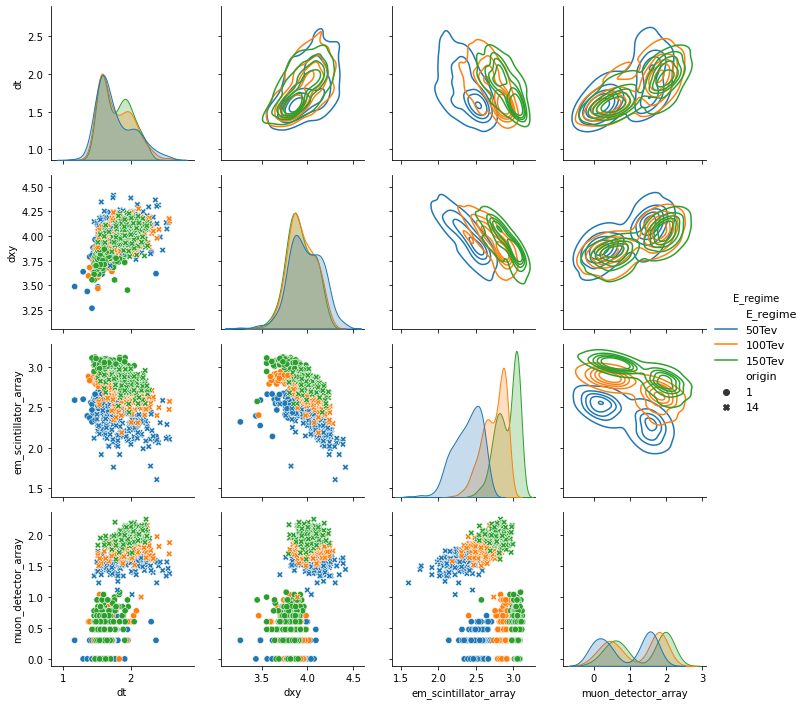
\includegraphics[width=0.9\textwidth]{imgs/data_exp_ener.png}
    \caption{Visualization of the information in the event master table with 900 showers (150 in each case of energy regime and primary particle).The separation between proton and photon induced showers is contrasted with the energy regime distributions in the space of features. }
    \label{fig:dataexploration_ener}
\end{figure}
\subsection{Event classification model}
The prediction model is built built to classify properly the particle showers, so that given a set of feature-target examples to train, the model can classify future events when providing the set of features observed. for the construction and evaluation of the models we will discuss the data set used is the complete data set of 1600 events.

An important consideration is to prioritize data availability. We discussed before that LHAASO can retrieve form each particle detection its approximate xy-coordinate and time of detection, but is convenient to assume that the only information retrieved is the detections itself. We will refer in future development the plane formed by the axes \emph{em\_scintillator\_array} and \emph{muon\_detector\_array} as the \textbf{counts space}, since its a subspace of the data. 

In this case of study, a simulation of LHAASO detection data, the goal is to classify this events as good as possible, but specifically to discard protons showers (PS).  LHAASO is interested in collecting gamma shower (GS) observations in order to map the \textit{Galactic diffuse gamma-ray emission} above few hundreds GeV, at new energy ranges. Then, a thing to have in mind when deciding a good classification model is that, in this case, is better to misclassify a few GS and discard them, than misclassifying some PS and having them into account as GS. In other words, when taking GS for astronomical studies is better to be \textit{picky} and have fewer data\footnote{We are also interested in maintaining this GS loss below certain threshold, so that a major percentage of the true GS are classified correctly} than having some wrong data. 

In the context of the binary classification itself, its worth reminding that the \textbf{recall} in this case is \textit{the fraction of PS that are correctly classified} and the \textbf{sensitivity} reflects \textit{the fraction of GS that are correctly classified}.In an equivalent way, $1-$recall is \textit{the fraction of PS that are misclassified} and $1-$sensitivity is \textit{the fraction of GS that are misclassified}. The last said, the correct direction to favor gamma ray astronomy is to prioritize the maximization of the recall at the cost of losing some sensitivity.

This case is a binary classification, so it is convenient to set the target value as a Boolean. since we want to detect specifically PS, this is going to be a  \textbf{positive case} (or 1), and GS are assigned as a \textbf{negative case} (or 0) respectively. This might be useful to check concepts like confusion matrix, sensitivity, recall, accuracy and F1 score.  



\subsubsection{Testing Models}

To decide which model could best fit the requirements of classification an exploratory analysis of the predictive models is executed over the counts space. Measurements of the classification performance were made to quantify the results, but in this case we are interested in two aspects: the shape of the boundary must be relatively soft (avoid overfitting) and the model can be modified to prefer one case of misclassification over the other.  The results of the tests are shown in figure \ref{fig:modeltest}. Its important to remark the good performance that all the methods had in the data, most all of them managed to find the boundary that divides the two clouds and in average have accuracies over 96\%. As an additional check, I wanted to see how the Random forest rank the importance of the features when classifying. The results available in figure \ref{fig:importances} confirm the observations in previous analysis where the muon detector counts and the time dispersion are the most relevant parameters in the classification of the target.  
\begin{figure}[!h]
    \centering
    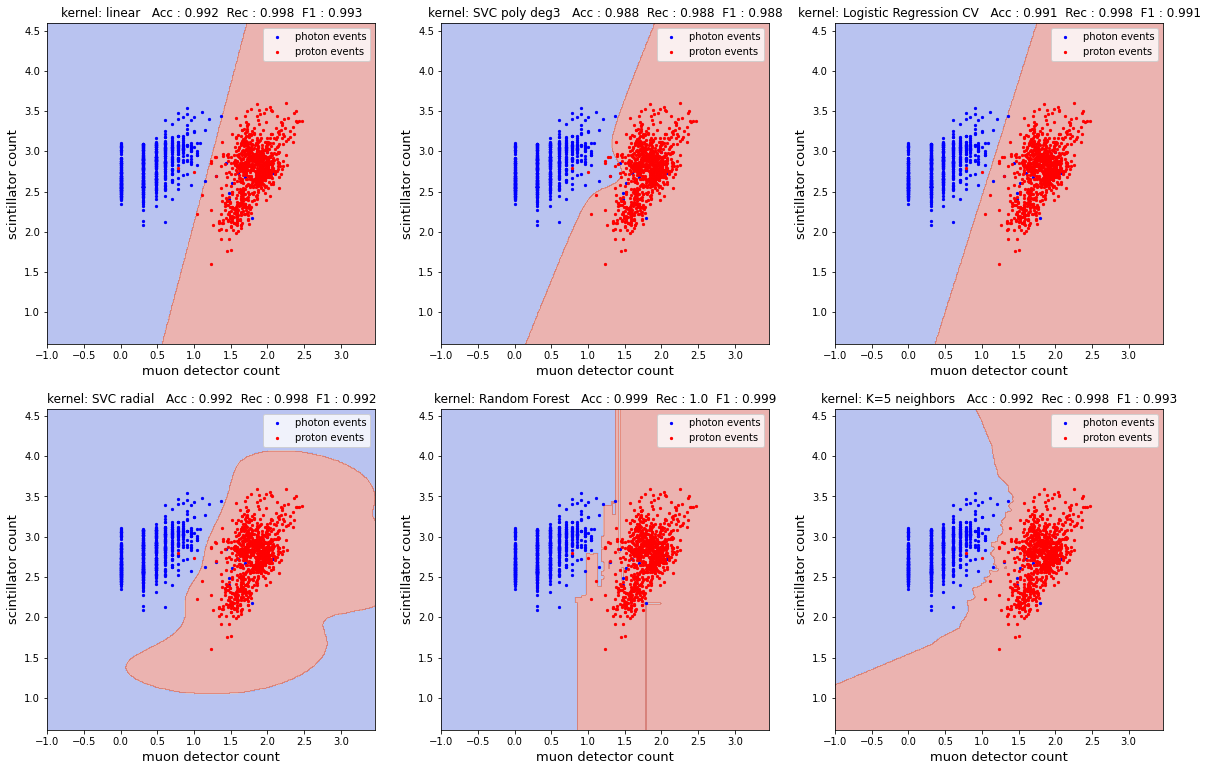
\includegraphics[width=\textwidth]{imgs/modeltest.png}
    \caption{Performance test over the counts space of Support vector Classifier (RBF kernel, C = 5), Random Forest (50 trees), lineal and polynomial (3 degree) regressors, Logistic Regression and K-nearest neighbors (5 neighbors). The accuracy, recall and F1 scores are measured in each classification test. }
    \label{fig:modeltest}
\end{figure}
After testing these models I chose to continue with a Logistic regression taking into account the following points:
\begin{itemize}
    \item Is a relatively simple classification model: this helps to understand totally the process behind and opens the possibility to assign physical meaning to the values that the model uses to classify
    \item Shows a good performance in the counts space and the boundary  of classification is consistent with the visible separation pattern
    \item Works by classifying values in the range [0,1] (obtained by the regression) according to a threshold value. This classification threshold value can be tuned by the user
    \item Can be reduced to a classification formula in which the coefficients of the regression can be obtained by training the model, and applied in the formula to classify new events.
    
\end{itemize}

\subsubsection{Logistic Function and probability threshold}
A Logistic regression is the predictive model chosen to classify the shower event data. This model can be seen as a linear combination of the features \textit{plugged} into a Logistic function. The linear combination range is the whole real numbers, but the logistic function maps this space into the [0,1] interval, reflecting the probability of the observation of being positive. Each new example is assigned to a real number according to the linear combination and eventually to a \textbf{probability}  between 0 and 1 of being a PS, this since the positive cases are reserved for this class. Then, the model defines a threshold (usually 0.5) to classify the events according to their probability. This threshold value can be tuned in order to satisfy the requirements of this classification, specifically to minimize the quantity $1-$recall.

By retrieving the probability, instead of the complete classification, one can define a threshold manually by defining the acceptable probability of being a PS needed to be classified as a PS. In order to do that I defined a \textbf{error assessment function} that, given the true target classes and the probabilities assigned by the model, can define the threshold value in order to minimize both quantities, $1-$sensitivity and $1-$recall, giving priority to the latter. These quantities are equivalent to \textit{fraction }This function is highly dependent in the data given since most of the times it selects as threshold the probability value of the PS example with less probability of being classified as PS. But even with this flaws, it can be trained through cross validation to obtain a more objective value for threshold.

The function works by splitting the interval [0,1] in $\sim10^{4}$ threshold value candidates, and starts sweeping them form lowest to highest, testing in each iteration the fractions of PS and GS that are misclassified, verifying that $1-$recall is below some \textbf{PS error tolerance} (set in $\sim10^{-4}$ in order to compare with the results obtained in \cite{UHEgammapaper}) and $1-$sensitivity is above some \textbf{GS loss tolerance} (even losing up to 50\% of GS information can be acceptable when the data is correct and the detections are numerous). If these conditions cannot be met, the threshold is set to 0.5 by default.


\begin{figure}[!h]
    \centering
    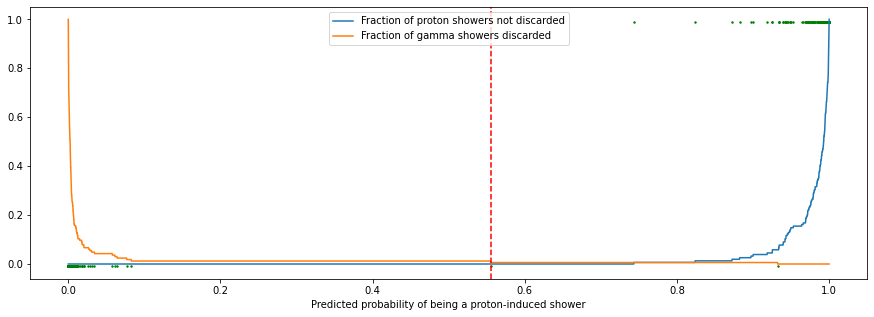
\includegraphics[width=\textwidth]{imgs/err_ass_th.png}
    \caption{Test of the error assessment function over the predicted probabilities of 1600 examples on a Logistic Regression classifier. The threshold found is 0.555 where 0.0\% of proton showers are misclassified and 0.61\% of gamma showers are miscalssified. The intercept an coefficients of the regressor are -0.76 and ( 6.3, -4.07,  2.2, -0.04) respectively, the order or the coefficients is (muon\_detector\_array, em\_scintillator\_array, dt , dxy). The green dots represent the real classes (y-axis) plotted against the predicted probability (x-axis).}
    \label{fig:err_ass_th}
\end{figure}

A test of the error assessment function was tested on a Logistic classifier as seen in figure \ref{fig:err_ass_th}. Observe that the threshold is not trivial, since intuition says it might be smaller than 0.5 but this is not the case. This is expected to change when feeding a larger volume of examples. In the figure we can see how well the Logistic classifier manages to separate the probabilities of the two groups, giving almost exclusive clusters. Note that even if the threshold moves back to 0.1 the percentage of misclassified gamma showers would be under 1\%.



\subsubsection{Pseudo-empiric Logistic classifier}
Let's have into account that a logistic Regression classification can be done only knowing the coefficients of the regression (one for each feature), the intercept and the threshold value. So given a sufficiently big set of data the Logistic regression classifier can be simplified into a semi-empirical formula for classifiying shower events.

With the purpose of making the process automatic, I created a script that provides the error function assessment and integrates it with a logistic regressor into a predictor object that can be trained, evaluated and, naturally, can predict the classes of new feature sets. This model when trained with the master table also generates the coefficients  needed to recreate the classifier i.e. a threshold $\tau$, an intercept $C_o$ and one coefficient $C_i$ for each feature of the master table. This is independent of the number of features, opening the possibility to evaluate a model with the whole table or one just with the counts space. Both models learn from the 1600 examples: they split the sample in train and test defined by a fractional \textbf{test size} value and train as a conventional model. When the test size is 0, the model is trained and evaluated over the whole data set. The results of this assessment is in Table \ref{tab:log_prob_test_size}



\section{Conclusions and Future Work}
High altitude Extensive Air Showers can be simulated with  MonteCarlo methods induced from theoretical models \cite{heitlerarticle} \cite{CORSIKA} obtaining results that are consistent with current theory and experimental data \cite{heitler1984quantum}. Moreover,
A simulation of in-ground detectors was developed successfully, recreating with acceptable accuracy the detector disposition in LHAASO as well as some of the observation conditions. The study of the difference between gamma rays and cosmic rays in the shower events agree with previous observations and theories:  the difference in muon count mentioned by other authors \cite{differencesgp} is noted as the most relevant parameter when trying to classify this events. The extensivity (or spatial dispersion) also shows a certain level of discriminant power over the shower events as mentioned before.

In the future it might be useful to study the dependence of the readings in the detector energy thresholds. This is useful to determine energy distributions among different detected particles and might as well give an insight of the relation of the master data with the energy regime. Also, in the future is recommended to extend the possibilities to more than showers coming form the zenith, but also from other directions and with centers not within the detector range. Independent of being a Toy model, assuming cosmic rays from all direction would give a more objective perspective on the master table data distributions.


In the counts space of the whole data table the clusters formed by the two different classes are well defined but not exclusive, meaning an accuracy of 100\% is nearly impossible. However, the recall can be maintained in 1 (or near) by moving the threshold according to the PS examples provided. This might affect the overall accuracy, but the cost in GS misclassification is low. The error assessment function coupled with the Logistic Regression Model satisfies the classification tests of shower event with more than 90\% accuracy, maintaining the PS error below $10^{-3}$ and the GS error below 15\%. The data available is not enough to replicate the results obtained by \cite{UHEgammapaper} in PS classification ($\epsilon_{PS} < 10^{-4} $), so a current objective is to optimize the event processing to generate a big enough master table.

The threshold definition can be better defined since the actual error assessment function is not an objective approximation of the distribution boundary. 

The dependence of the counts space data in the energy of the primary particle is expected from physical intuition an can be approximated through the Heitler model of particle showers\cite{heitlerarticle}. A possible advance in this direction could be generating a model that can predict the primary particle and its energy range according to the data in the master table.

This model allowed the use of a semi-empiric formula for classifying future data sets, simplifying the process and can be modified to output the probability values before the threshold classification into other model with more input data. A current proposal is to mix the results obtained in this \textit{Toy Model} with the use of convolutional neural networks for image recognition in the spatial detection patterns to give a better result given what we understand now about EAS\cite{charsEAS}. Combining the two methods would not be sophisticated since is still approaching the problem without all the real considerations, but would show how the CNN data could relate with the distributions in the counts space to enhance more sophisticated algorithms. 




\newpage

\bibliography{reference}
\bibliographystyle{ieeetr}


\newpage
\begin{appendices}

\section{CORSIKA} 
\subsection{Input file}
\label{filecorsika}
This input file corresponds to an example of 1000 proton induced showers, with energy range limits and energy slope defined by \emph{ERANGE} and \emph{ESLOPE} respectively.
\begin{lstlisting}[basicstyle=\tiny]
RUNNR 4 number of run [to name the file]
EVTNR 100400 no of first shower event 
SEED 100411 0 0 seed for hadronic part
SEED 100412 0 0 seed for EGS4 part
SEED 100413 0 0 seed for Cherenkov part
NSHOW 1000 no of showers to simulate
PRMPAR 14 primary particle code (iron) [14 for proton showers]
ERANGE 5.E3 5.E5 energy range of primary (GeV) 
ESLOPE -2.7 slope of energy spectrum
THETAP 0. 0. range zenith angle (deg) [particles coming from the zenit]
PHIP -180. 180. range azimuth angle (deg) [all azimuthal angles]
HADFLG 0 0 0 0 0 2 HDPM interact.flags & fragmentation flag
ELMFLG T T elmag. interaction flags NKG, EGS4
STEPFC 1. multiple scattering step length factor
RADNKG 200.E2 outer radius (cm) of NKG elect. distrib.
MAGNET 20.4 43.23 magnetic field central Europe (/uT)
ECUTS .3 .3 .015 .015 energy cuts: hadr. muon elec. phot. (GeV)
LONGI T 20. T T longitud, stepsize(g/cm2), fit, out
MUMULT T muon multiple scattering by Moliere
MUADDI T additional muon information
OBSLEV 44.E4 observation level (cm)
ARRANG 18.25 angle between north to array-grid (deg)
MAXPRT 10 max. no of printed events
ECTMAP 1.E2 printout gamma factor cut
DIRECT /[PATH]]/  directory of particle output
DATBAS T write data base file
USER you user name for data base file
DEBUG F 6 F 999999999 debug flag, log. unit, delayed debug
EXIT
\end{lstlisting}

\subsection{DANTE Performance}
\begin{figure}[!h]
    \centering
    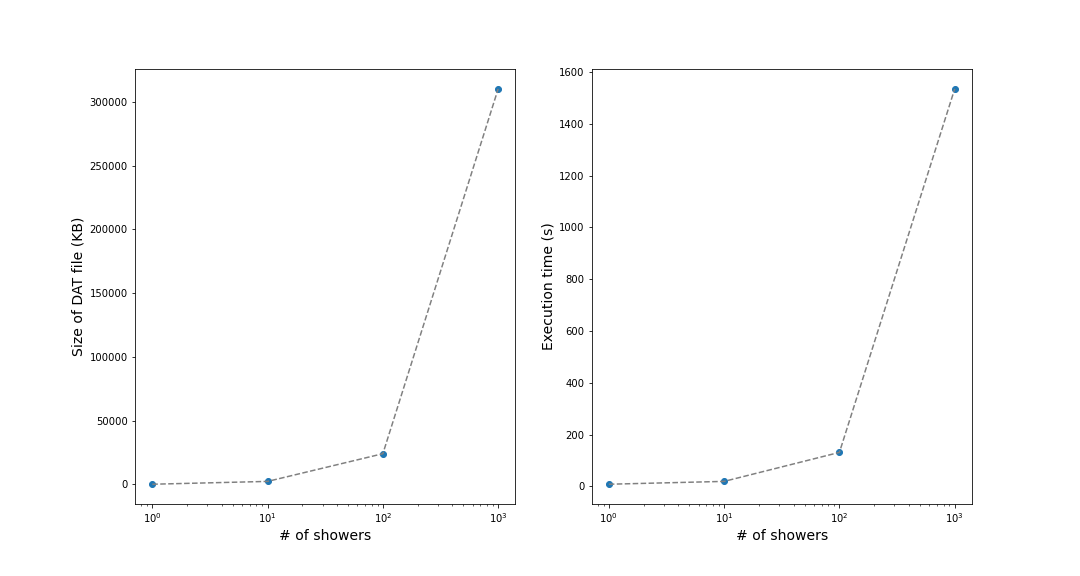
\includegraphics[width=\textwidth]{imgs/corsikaDantePerformance.png}
    \caption{performance information of DANTE cluster at APC. The process was executed in one node of 40 processors. It´s important to mention that with the increase of initial energy the number of particles generated in the shower increases and eventually the number of calculations increase exponentially. When generating the 150 shower batches, the time needed for the 150TeV events increased drastically. }
    \label{fig:DANTEperformance}
\end{figure}

\newpage
\section{LHAASO}
\subsection{Design}
\begin{figure}[!h]
    \centering
    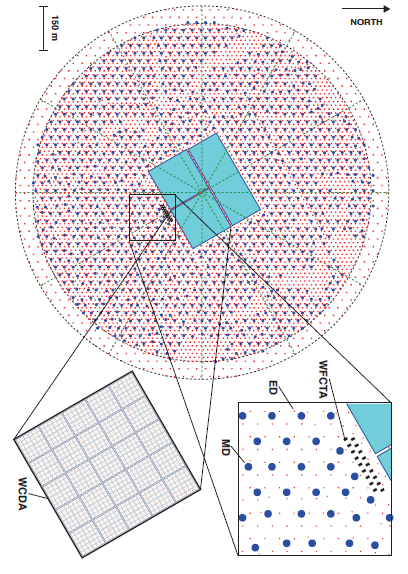
\includegraphics[width=0.6\textwidth]{imgs/detect_array_lhaaso_paper.PNG}
    \caption{According to the LHAASO paper \cite{LHAASOpaper}, this is the   distribution of Electromagnetic Detectors (EM), Muon Detectors(MD), wide field-of-view air Cherenkov telescopes (WFCTA) and water cherenkov Detectors (WCDA).  The inner and outer circles have a radius of 575m and 635m respectively. The inner circle specifications were used to build the simulated detector array discussed in figure \ref{fig:detectorarray}. }
    \label{fig:lhaasodesign}
\end{figure}

\newpage
\section{Data and modeling}
\subsection{Correlations and covariances}
 \begin{figure}[!h]
    \centering
    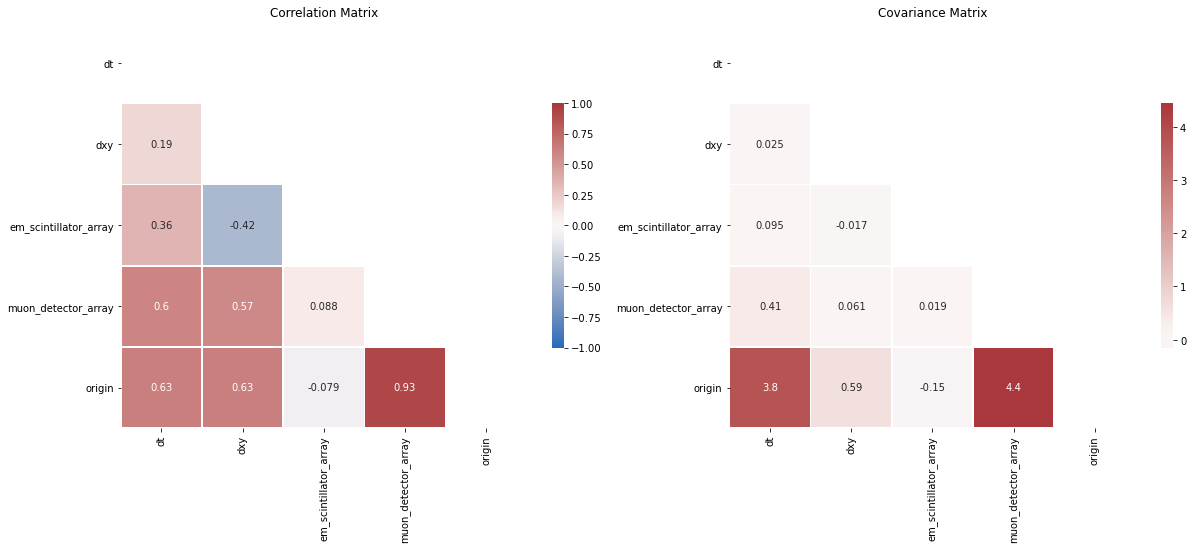
\includegraphics[width=\textwidth]{imgs/covcorr.png}
    \caption{Representation of the covariance and correlation among different columns in the master table. Covariance is a positive number while correlation is a number in [0,1].}
    \label{fig:covcorr}
\end{figure}
 \begin{figure}[!h]
    \centering
    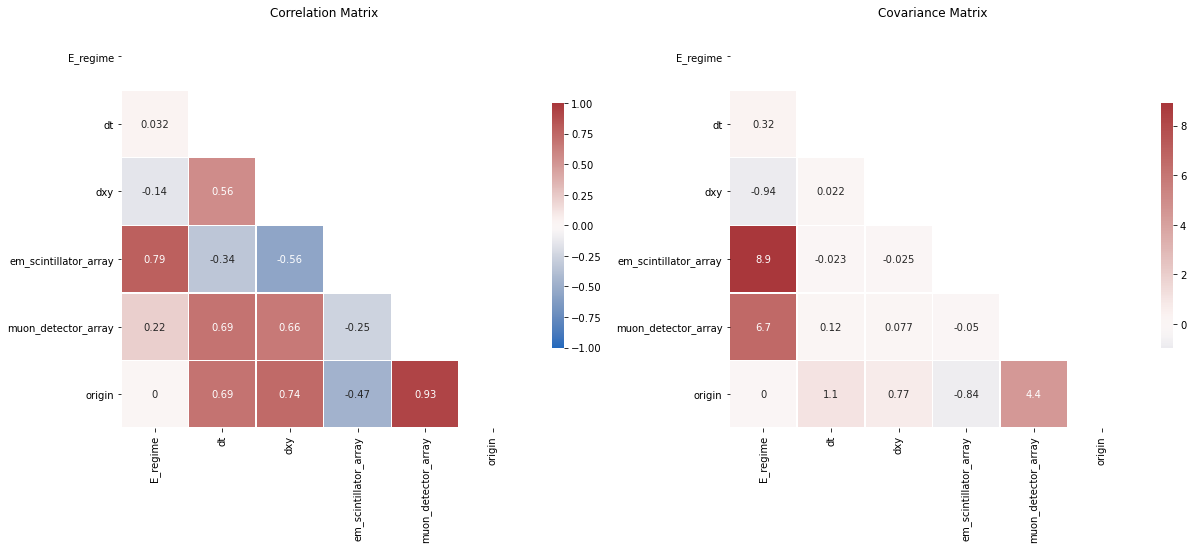
\includegraphics[width=\textwidth]{imgs/covcorr_ener.png}
    \caption{Representation of the covariance and correlation among different columns in the master table when checking different energy regimes. The correlation zero and covariance zero between \emph{origin} and \emph{E\_regime} is a consequence of the balanced data set, with real measurements this values might change implying a relation between energy of the primary particle and its type.}
    \label{fig:covcorr_ener}
\end{figure}
\newpage
\subsection{PCA}
The basis of the plane of projection is given by the components described in Table . The mean value is an additive constant that contains the bias of non-normalized data (under the assumption of normality).
\begin{table}[h!]
\centering
\begin{tabular}[]{c|cccc}
\hline
    & \textbf{muon\_detector\_array} & \textbf{em\_scintillator\_array} & \textbf{dt} & \textbf{dxy}  \\
  \hline
  \hline
  \textbf{First component} & 0.556 & 0.081 & 0.826 & 0.046 \\
  \textbf{Second component} & -0.809 & 0.195 & 0.534 & -0.151\\
  \textbf{Mean} & 1.106 & 2.782 & 2.199 & 3.916\\
  \hline
\end{tabular}
    \caption{Principal components an mean for the projection in Figure \ref{fig:pca}.}
    \label{tab:pcacomp}
\end{table}
\begin{figure}[!h]
    \centering
    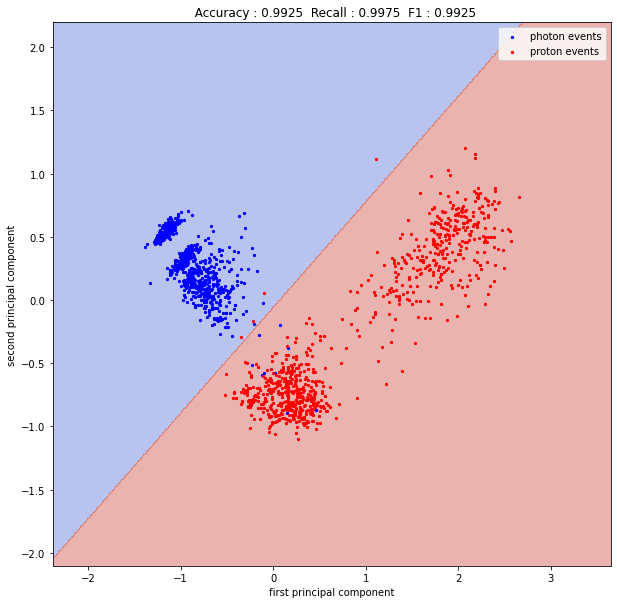
\includegraphics[width=\textwidth]{imgs/pca.png}
    \caption{1600 showers in the 4-dimensional space of features from the master table. This space is projected over the plane that maximizes the variance of data when projected. A Logistic Regression is trained on the 2D data points, and split the plane in two classification regions.}
    \label{fig:pca}
\end{figure}
\newpage
\subsection{Random Forest importances}
\begin{figure}[!h]
    \centering
    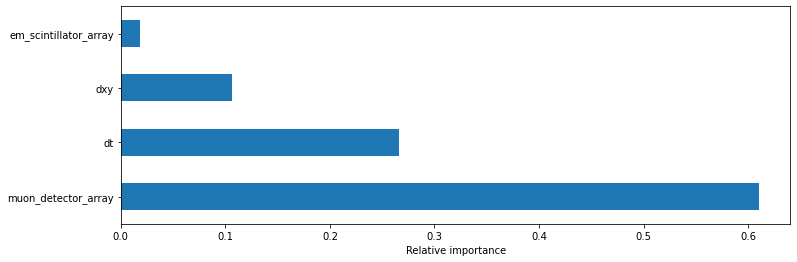
\includegraphics[width=0.9\textwidth]{imgs/importRF.png}
    \caption{Relative importances according to a Random Forest Classifier with 100 trees.}
    \label{fig:importances}
\end{figure}

\subsection{Logistic Model coefficients and performance}
\begin{table}[!h]
\centering
\begin{tabular}[]{l|ccc|ccc}
\hline
  & \multicolumn{3}{c}{Complete}  & \multicolumn{3}{c}{Counts space} \tabularnewline
\hline
Test size    & \textbf{0\%} &\textbf{15\%} & \textbf{30\%} & \textbf{0\%} & \textbf{15\%} &\textbf{30\%}  \\
  \hline
  $\tau$ & 0.272 &	0.351 &	0.332 & 0.214 &	0.215 &	0.362\\
  $C_o$ &-8.568 &	-5.742	& -5.409 &-2.376	&-2.395 &	-2.215   \\
  $C_{EM}$ & 4.88	& 2.816 &	2.635  & -0.6 &	-0.526 & -0.493  \\
  $C_{MD}$ &  -1.95	& -0.77 &	-0.707 & 0.946 &	0.944 &	0.985  \\
  $C_{\Delta t}$ & 1.764	& 1.187 & 1.146   & - & - & - \\
  $C_{\Delta xy}$ &  1.18 & 0.573 &	0.518 &  - & - & -   \\
  \hline
  Acc.   & 99.3\% &	99.1\% & 99\% & 94\%	& 95\% &	98.5\%     \\
    F1 & 0993 & 0.992 &	0.99 &  0.946 &	0.944 &	0.985 \\
  $\epsilon_{PS}$ &  0\%	& 0\%	& 0\% & 0\% &0\% & $\sim$ 0.1\% \\
    $\epsilon_{GS}$ &  1.3\% &	1.6\% &	2\%  & 10.7\% & 11.1\% & 2.8\% \\
  \hline
  
\end{tabular}

\caption{Evaluation of the logistic threshold model (with the error assessment function) in complete master table vs. only the count space with different test sample sizes. The coefficients for each feature, the threshold and the intercept are displayed as well as some metrics: accuracy, F1 score, proportion of misclassified PS to the total true PS and the same error metric  for GS. These values are obtained through a 10 batch cross validation, with a relatively low variance among batches. }
\label{tab:log_prob_test_size}
\end{table}
\section{Code}
The commented code and notebooks used for this stage report and the analysis made is available on \textbf{github.com/PaipaPsyche/stageAPC}
The organization and content of the repository is: 
\begin{itemize}
    \item \textbf{file\_processing} management and decryption of CORSIKA output files, EAS particle distributions, example of use of LHAASO grid simulator.
    \item \textbf{performance} CORSIKA input files, Generation of CORSIKA output files, DANTE performance. 
    \item \textbf{MLclassification} Testing different models, building the master table, exploratory analysis of master table, Proposal of PCA and threshold logistic regressor, performance evaluation of models.
    \item \textbf{shower\_data} master tables used in the development of this study.
    \item \textbf{energy\_exploration} studying the energy regime influence in the master table
\end{itemize}
\end{appendices}

\end{document}